\documentclass[sigconf]{acmart} 

% --- Encoding and Fonts ---
\usepackage[utf8]{inputenc} 
\usepackage[T1]{fontenc} 
\usepackage{lmodern} 

% --- Table Packages ---
\usepackage{tabularx} 
\usepackage{array} 
\usepackage{caption} 

% --- Optional but recommended for academic papers ---
\usepackage{hyperref} 
\usepackage{booktabs} 

\usepackage{subcaption}

\begin{document}

\newcommand{\displayimages}[9]{
\begin{figure}[h]
    \centering

    \begin{subfigure}{0.49\columnwidth}
        \includegraphics[width=\linewidth]{../generated-videos/API/frames/#1_0000#5_/#1_0000#5__02.jpg}
        \caption{#6}
    \end{subfigure}
    \hfill
    \begin{subfigure}{0.49\columnwidth}
        \includegraphics[width=\linewidth]{../generated-videos/API/frames/#2_0000#5_/#2_0000#5__02.jpg}
        \caption{#7}
    \end{subfigure}

    \vskip\baselineskip

    \begin{subfigure}{0.49\columnwidth}
        \includegraphics[width=\linewidth]{../generated-videos/API/frames/#3_0000#5_/#3_0000#5__02.jpg}
        \caption{#8}
    \end{subfigure}
    \hfill
    \begin{subfigure}{0.49\columnwidth}
        \includegraphics[width=\linewidth]{../generated-videos/API/frames/#4_0000#5_/#4_0000#5__02.jpg}
        \caption{#9}
    \end{subfigure}

    \caption{Prompt #5}
\end{figure}
}

\title{A Survey: Video Generative Models}

\author{Taraash Mittal}
\authornote{Both authors contributed equally to this research.}
\email{taraash23552@iiitd.ac.in}

\author{Utkarsh Garg}
\authornotemark[1]
\email{utkarsh23570@iiitd.ac.in}

\author{Anoop Ratn}
\author{Rajiv Ratn Shah}
\affiliation{%
    \institution{Indraprastha Institute of Information Technology}
    \city{Delhi}
    \country{India}
}

\renewcommand{\shortauthors}{Mittal and Garg, et al.}

\begin{abstract}
    The rapid evolution of generative artificial intelligence has positioned video generation as the current frontier of creative machine learning models. Despite a recent burst of such architectures, there remains a notable absence of large-scale comparative studies analyzing their practical capabilities. This paper addresses this gap by first underpinning the general inner workings of video generative models, followed by a detailed examination of the unique functional mechanics of each model evaluated in this study[cite: 15]. To systematically assess these systems, we introduce a curated list of targeted stress-testing prompts designed to rigorously judge the models' temporal coherence, spatial and physical reasoning, prompt inference accuracy, and animation style lineage. The detailed methodology and prompt list are described in Section \ref{sec:targeted_and_stress_testing}. Ultimately, we comprehensively review the current state of both open-source and premium AI generative video models across a variety of use cases, explicitly testing their individual strengths and weaknesses to evaluate their viability in professional workflows[cite: 18]. The complete generated dataset, facilitating further research and reproducibility, can be found on the author's \href{https://www.github.com/T-Cent/Character-Consistency}{GitHub}.
\end{abstract}

\begin{teaserfigure}
    \centering
    
\includegraphics[height=15em]{images/image.png}
    % \vspace{0.1\textwidth}
    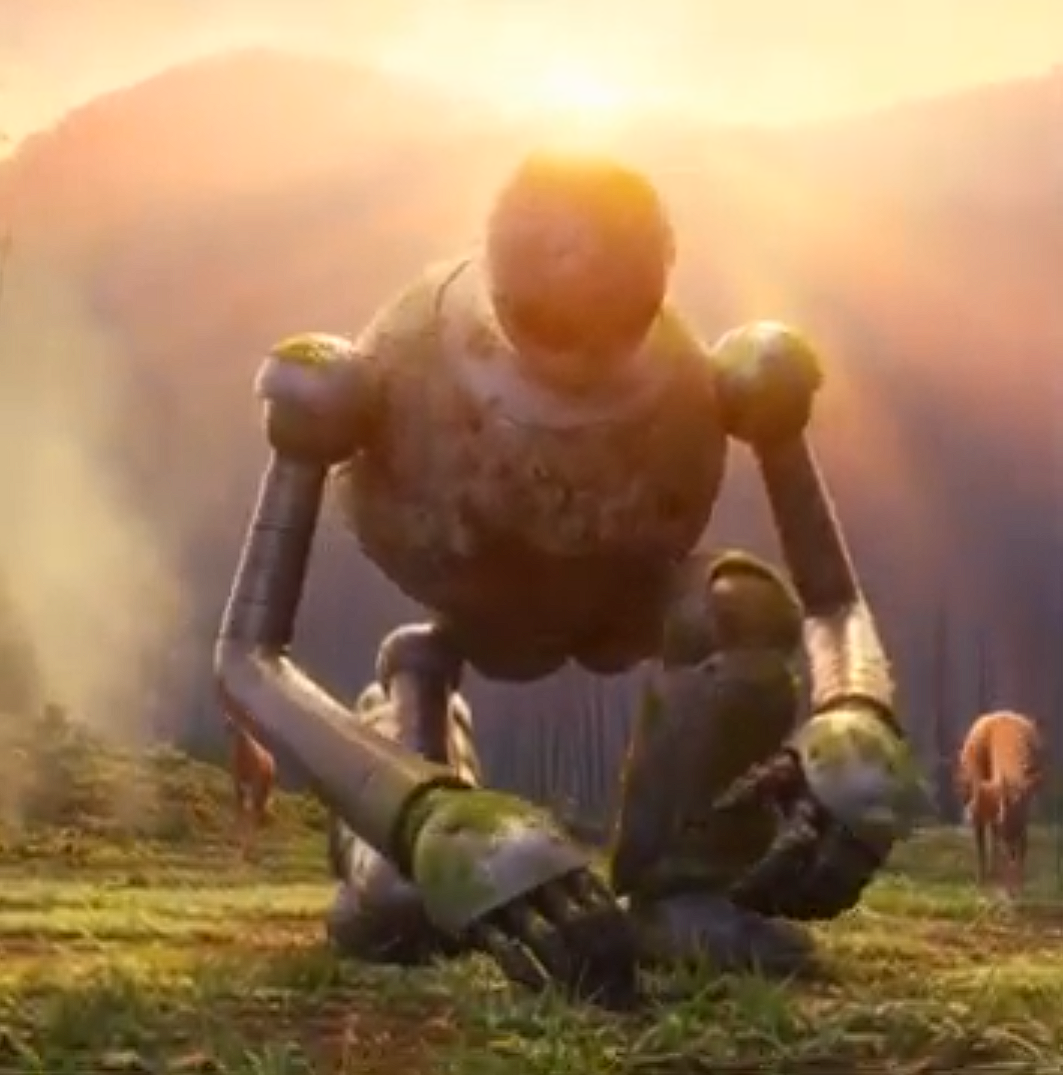
\includegraphics[height=15em]{image.png}
    \caption{Wild Robot (left: real; right: extended using Wan 2.2)}
\end{teaserfigure}

\maketitle

\section{Introduction}

As is the current landscape of Generative AI, one can immediately go online and have an AI generate any video they want, given a text and/or an image, largely free of cost. The quality of such videos is usually not what the user originally had in mind, but the current state-of-the-art (SOTA) models have been able to provide videos of reasonably high quality. Additionally, there has been much development from the open-source community to ``catch-up'' to the quality provided by the closed-sourced competitors. The ability to generate complex temporal media through prompt engineering represents a massive shift in creative workflows, bringing rapid prototyping to cinematography. However, integrating these models into professional pipelines requires them to adhere strictly to human instructions and maintain physical and spatial consistency across generated frames.

Despite impressive visual fidelity, current generative architectures face significant mechanical and spatial challenges. Models frequently struggle with object permanence and structural integrity; for instance, high-frequency details often exhibit slight 2.5D warping at macro scales rather than maintaining true 3D fabric persistence. Temporal consistency remains a major hurdle, as models often cannot maintain object permanence or texture stability during a simple vertical drop.

When tasked with simulating gravity or complex interactions, models can fail entirely, sometimes resulting in catastrophic physics failures. A prime example is "object mitosis," where the model completely loses track of an object's geometry and mass, causing a single item (like a bouncing ball) to erroneously split into two. Even basic Newtonian physics, such as simulating elastic rebounds or kinetic energy transfer, can cause models to fail. In long-horizon coherence tests, instead of rendering continuous action, models frequently hallucinate new states or rely on severe jump cuts.

To systematically evaluate these capabilities, we devised a strong set of prompts to judge various \emph{types} of video and how individual models perform at each such genre. We categorize these into metric-specific baselines, stylistic baselines, and advanced stress tests. Our evaluation covers a diverse array of SOTA models, specifically:
\begin{enumerate}
    \item Grok
    \item Kling O3
    \item LTX 2.6
    \item Seedance 1.5
    \item Veo
    \item Vidu Q3
    \item Wan 2.2 \footnote[1]{Run locally on a single 4080 SUPER}
    \item LTX 2 \footnotemark[1]
\end{enumerate}

Our metric baselines isolate specific mechanical parameters. For example, the "Red Cube" prompt (Prompt [1]) evaluates whether a primitive geometric shape can maintain its absolute structural and color integrity during continuous, smooth camera translation without morphing or flickering. The "Rubber Ball" prompt (Prompt [2]) assesses the model's understanding of basic Newtonian physics, specifically gravity, elasticity, momentum preservation, and kinetic energy decay upon contact with a rigid surface. For advanced stress tests, we introduced scenarios like the "Tea Sequence" (Prompt [6]) to evaluate logical narrative sequencing; it challenges the model to link distinct, sequential actions into a cohesive timeline without skipping steps or forgetting the initial context. Furthermore, we tested stylistic adherence, such as prompting for an anime-style cat (Prompt [C]) to gauge the model's understanding of specific Japanese animation tropes, including distinct shading techniques, exaggerated proportions, and potential modulation of perceived frame rates.

In this paper, we review the current state of open-source and premium AI generative video models on a variety of use cases and test their strengths and weaknesses through various curated prompts. Crucially, other works never tested this many models and never on the breadth of testing criteria. We first give a high-level overview of how these models function in general, previously using Variational Autoencoders and Generative Adversarial Networks. We then describe Diffusion Transformers, the technology that powers the current SOTA models.

The accompanying GitHub repository can be found on the author's \href{https://www.github.com/T-Cent/Character-Consistency}{GitHub}. The dataset can be found on \href{https://drive.google.com/drive/folders/1cEVKn6BVKXk5Svhe4l1FFPjY2MZcX6lc?usp=sharing}{Google Drive}, which also contains results of preliminary testing and exploration.

\section{Background and Related Work}
\label{sec:background}

The landscape of Generative Artificial Intelligence (AI) for video synthesis has evolved rapidly, transitioning from early exploratory architectures to massive, data-driven foundation models \cite{kaswan2023generative, xie2025comprehensive}. To contextualize the models evaluated in this study, it is crucial to understand the underlying architectures and how they generate high-dimensional spatio-temporal data under the hood.

\subsection{Foundational Generative Architectures}
Early approaches to text-to-video (T2V) generation relied predominantly on Variational Autoencoders (VAEs) and Generative Adversarial Networks (GANs) \cite{kaswan2023generative, xie2025comprehensive}.
\begin{itemize}
    \item \textbf{VAEs:} These models consist of an encoder that maps input data into a probability distribution and a decoder that generates new data by sampling from this learned distribution \cite{xie2025comprehensive}. While structurally simple, VAEs often suffer from "posterior collapse" and struggle to generate highly complex, high-resolution videos \cite{xie2025comprehensive}.
    \item \textbf{GANs:} Generative Adversarial Networks operate via an adversarial process between a generator and a discriminator \cite{xie2025comprehensive}. While capable of producing images with good perceptual quality, GANs frequently suffer from pattern (mode) collapse and struggle to scale to complex, large-scale video datasets with diverse human movements \cite{xie2025comprehensive}.
\end{itemize}

To overcome these limitations, the field shifted toward \textbf{Autoregressive Transformers}. These models generate video sequences in a step-by-step manner, where the latest generated content is conditioned on previously generated frames \cite{xie2025comprehensive}. This natural fit for sequential data avoids GAN pattern collapse and yields higher video quality, albeit at the cost of massive computational and memory resources \cite{xie2025comprehensive}.

\subsection{Under the Hood: Diffusion Models and DiT}
The current generation of state-of-the-art commercial models (including the architectures powering Sora, Veo, Kling, and others evaluated in this paper) are predominantly built upon \textbf{Diffusion Models} and \textbf{Diffusion Transformers (DiT)}.

At its core, a Denoising Diffusion Probabilistic Model (DDPM) learns to synthesize data by first adding random Gaussian noise to existing data over a series of steps, and then training a neural network to reverse this process (denoising) to recover the high-quality image or video \cite{xie2025comprehensive}. Because operating directly in pixel space is computationally prohibitive for video, modern models utilize \textbf{Latent Diffusion}. In this approach, an encoder maps the video into a highly compressed latent representation, the diffusion process occurs within this smaller latent space, and a decoder reconstructs the final video pixels, significantly reducing computational consumption \cite{xie2025comprehensive}.

Recently, the traditional U-Net backbones used in diffusion models have been replaced by Transformers, creating the \textbf{Diffusion Transformer (DiT)} architecture \cite{xie2025comprehensive}. Models utilizing DiT (such as OpenAI's Sora) exhibit several advanced capabilities under the hood:
\begin{enumerate}
    \item \textbf{Variable Resolution Training:} They can be trained natively on videos and images of varying resolutions, durations, and aspect ratios without extreme cropping \cite{xie2025comprehensive}.
    \item \textbf{Prompt Expansion:} They leverage Large Language Models (LLMs) to automatically convert short, vague user prompts into highly detailed instructions, drastically improving the semantic alignment and quality of the generated video \cite{xie2025comprehensive}
\end{enumerate}

\subsection{The Necessity of Stress Testing}
Traditionally, T2V models are evaluated using automated quantitative metrics such as Fréchet Video Distance (FVD) and Inception Score (IS) for visual quality, alongside CLIPSIM for text-video semantic alignment \cite{xie2025comprehensive}.

However, recent studies indicate that these automated evaluation metrics often misalign with actual human judgments and fail to capture nuanced failures in temporal consistency, physics, and complex motion \cite{xie2025comprehensive}. Consequently, qualitative assessment and rigorous human evaluation remain essential \cite{xie2025comprehensive}. To bridge this gap, our methodology eschews broad automated metrics in favor of highly targeted, fine-grained stress-testing prompts designed to isolate specific mechanical, spatial, and temporal capabilities.

\section{Targeted Prompts and Stress Testing Methodology} \label{sec:targeted_and_stress_testing}
To isolate specific failure modes and evaluate foundational capabilities, we utilize a set of targeted prompts designed to test exactly one domain at a time.
This provides a neutral baseline before introducing complex, multi-layered scenarios. We categorize these into metric-specific baselines, stylistic baselines, and advanced stress tests.

\subsection{Dataset Creation}

We briefly describe our generation pipeline and prompts used.

To facilitate locally run models, we set up ComfyUI on a Windows machine using an NVIDIA 4080 Super and an Intel i7 chip. We then devised three ``categories'' of prompts:
\begin{enumerate}
    \item Testing/baseline prompts: they are extremely simple and direct prompts, testing exactly one thing, such as \begin{enumerate}
              \item Temporal consistency
              \item Spatial awareness
              \item Physical interactions
              \item And more...
          \end{enumerate}
    \item Animation styles: to judge what type of videos a particular model can create, we categorized these into:
          \begin{enumerate}
              \item cartoon
              \item anime (exaggerated animation)
              \item realistic
              \item hyper-realistic
              \item educational
          \end{enumerate}
    \item Creative prompts: Actual, real-world prompts and use cases
          \begin{enumerate}
              \item extending a video
              \item generating a video from an image
              \item a complex video from text
          \end{enumerate}
\end{enumerate}

\subsection{Targeted Prompts: Metric Baselines}
These prompts isolate individual mechanical, spatial, or temporal capabilities of the video generation models.

\begin{itemize}
    \item \textbf{Prompt [1]:} ``A single red cube sits on a white table in a well-lit room. The camera slowly moves in a small circle around the cube. The cube does not change shape, size, or color at any point.''
          \\ \textbf{Testing:} Temporal consistency [1].
          \\ \textbf{How:} Evaluates whether a primitive geometric shape can maintain its absolute structural and color integrity during continuous, smooth camera translation without morphing or flickering.

          \displayimages{Grok}{kling_o3_t2v}{ltx-t2v}{seedance}{1}{Grok}{Kling}{LTX}{Seedance}


    \item \textbf{Prompt [2]:} ``A blue rubber ball is dropped from a height onto a flat concrete floor. The ball bounces several times, with each bounce reaching a lower height than the previous one, following realistic motion.''
          \\ \textbf{Testing:} Motion realism [2], Object interaction \& physics reasoning [7].
          \\ \textbf{How:} Assesses the model's understanding of basic Newtonian physics, specifically gravity, elasticity, momentum preservation, and kinetic energy decay upon contact with a rigid surface.

          \displayimages{veo}{kling_o3_t2v}{ltx-t2v}{seedance}{2}{Google Veo}{Kling}{LTX}{Seedance}


    \item \textbf{Prompt [3]:} ``A stationary wooden chair is placed in the center of a room. The camera performs a smooth forward dolly movement toward the chair without shaking or sudden jumps.''
          \\ \textbf{Testing:} Camera behavior [3].
          \\ \textbf{How:} Isolates virtual camera operation to determine if the model can execute a clean spatial translation (a dolly in) without inducing artificial camera shake, spatial warping, or dropped frames.

    \item \textbf{Prompt [4]:} ``A white sphere is placed on a flat surface under a single fixed overhead light source. The camera remains still. The lighting and shadows remain consistent throughout the scene.''
          \\ \textbf{Testing:} Lighting stability [4].
          \\ \textbf{How:} Tests the rendering engine's ability to hold a static lighting state, ensuring that the gradient shading on the sphere and the cast shadow on the surface do not swim or shift over time.

    \item \textbf{Prompt [5]:} ``A person wearing a plain green shirt and black pants walks in a straight line across a neutral background. Their appearance, clothing, and body proportions remain consistent throughout the video.''
          \\ \textbf{Testing:} Character preservation [5].
          \\ \textbf{How:} A fundamental locomotion test checking if human anatomy, limb proportions, and specific clothing colors remain stable during a repetitive biomechanical cycle (walking).


    \item \textbf{Prompt [6]:} ``A person enters a room, walks to a table, picks up a cup, and takes a sip. The sequence of actions should be clear and logically ordered.''
          \\ \textbf{Testing:} Prompt inference and context [6], Long-horizon coherence [10].
          \\ \textbf{How:} Evaluates logical narrative sequencing. It challenges the model to link distinct, sequential actions into a cohesive timeline without skipping steps or forgetting the initial context.

          \displayimages{vidu_q3_t2v}{veo}{ltx-t2v}{seedance}{3}{Vidu}{Google Veo}{LTX}{Seedance}


    \item \textbf{Prompt [7]:} ``A hand pushes a glass across a table. The glass slides, slows down due to friction, and stops.''
          \\ \textbf{Testing:} Object interaction \& physics reasoning [7].
          \\ \textbf{How:} Tests the transfer of kinetic force from an organic subject to a rigid object, and evaluates the model's simulation of friction and gradual deceleration.

    \item \textbf{Prompt [8]:} ``Three identical spheres (red, blue, and green) roll forward at the same speed across a flat surface without changing color or size.''
          \\ \textbf{Testing:} Multi-agent coordination [8], Temporal consistency [1].
          \\ \textbf{How:} Evaluates the ability to independently track multiple distinct entities moving in parallel. It tests whether the model suffers from color bleeding, merging, or varied acceleration between identical shapes.

    \item \textbf{Prompt [9]:} ``A person walks behind a large box and then reappears on the other side. Their appearance remains consistent.''
          \\ \textbf{Testing:} Spatial reasoning \& geometry [12], Character preservation [5].
          \\ \textbf{How:} A strict test of object permanence and occlusion handling. It determines if the model retains character identity and spatial trajectory while the subject is entirely hidden from the camera's view.

    \item \textbf{Prompt [10]:} ``A person wearing a shirt with thin horizontal stripes stands still while the camera slowly zooms in. The stripe pattern remains stable.''
          \\ \textbf{Testing:} Fine-grained detail consistency [9], Camera behavior [3].
          \\ \textbf{How:} Challenges the model with high-frequency textures during scaling. It evaluates resistance to aliasing, moir\'e patterns, and texture "swimming" as focal length changes.

          \displayimages{Grok}{kling_o3_t2v}{ltx-t2v}{seedance}{4}{Grok}{Kling}{LTX}{Seedance}


    \item \textbf{Prompt [11]:} ``A cube is placed in front of a sphere. The camera moves sideways, clearly showing that the cube remains closer to the camera than the sphere.''
          \\ \textbf{Testing:} Spatial reasoning \& geometry [12].
          \\ \textbf{How:} Tests depth perception and parallax rendering, ensuring the model understands 3D spatial layout and relative object positioning during lateral camera movements.

    \item \textbf{Prompt [12]:} ``A sign with the text ``OPEN'' is placed on a wall. The camera slowly moves closer while the text remains clear and readable.''
          \\ \textbf{Testing:} Text rendering [13].
          \\ \textbf{How:} Evaluates typographic stability. It tests if alphabetical characters maintain their structural geometry and legibility without morphing into unreadable symbols during camera motion.
\end{itemize}

\subsection{Targeted Prompts: Animation Styles}
These prompts utilize identical actions to isolate and evaluate the model's ability to adhere strictly to specified visual aesthetics and rendering techniques.

\begin{itemize}
    \item \textbf{Prompt [A]:} ``A cat walks from left to right across a room.''
          \\ \textbf{Testing:} Base style generation [A].
          \\ \textbf{How:} Establishes the model's default, unprompted output baseline for lighting, texture, and motion prior to any stylistic constraints.

    \item \textbf{Prompt [B]:} ``A cartoon-style cat walks from left to right across a room. The shapes are simple and stylized, with clean outlines.''
          \\ \textbf{Testing:} Cartoon and stylized [B].
          \\ \textbf{How:} Evaluates adherence to traditional 2D/3D western animation aesthetics, checking for flat shading, simplified geometry, and deliberate line work.

          \displayimages{Grok}{kling_o3_t2v}{ltx-t2v}{seedance}{5}{Grok}{Kling}{LTX}{Seedance}


    \item \textbf{Prompt [C]:} ``An anime-style cat walks from left to right across a room. The design uses exaggerated stylization typical of anime.''
          \\ \textbf{Testing:} Anime [C].
          \\ \textbf{How:} Tests the model's understanding of specific Japanese animation tropes, including distinct shading techniques, exaggerated proportions, and potential modulation of perceived frame rates.

    \item \textbf{Prompt [D]:} ``A realistic cat walks from left to right across a room. The scene uses natural lighting and believable textures.''
          \\ \textbf{Testing:} Realistic/cinematic [D].
          \\ \textbf{How:} Checks for accurate organic texture generation (fur), believable lighting environments, and true-to-life biomechanical motion.

    \item \textbf{Prompt [E]:} ``A highly detailed, photo-realistic cat walks from left to right across a room. The lighting, textures, and motion appear lifelike.''
          \\ \textbf{Testing:} Hyper-realistic/photo-real [E].
          \\ \textbf{How:} Pushes the realistic baseline to its limits, testing micro-details, complex light scattering, and absolute fidelity to real-world camera sensors.

    \item \textbf{Prompt [F]:} ``A simple educational-style animation shows a cat walking from left to right across a room, clearly illustrating the motion.''
          \\ \textbf{Testing:} Educational [F].
          \\ \textbf{How:} Assesses the ability to abstract visual information for clarity, potentially utilizing diagrammatic layouts or highlighted motion paths typical of instructional media.
\end{itemize}

\subsection{Stress Testing Prompts}
These prompts combine multiple domains, testing the absolute limits of the model's coherence over extended durations and complex interactions.

\begin{itemize}
    \item \textbf{Stress Test 1:} ``A person prepares a cup of tea from start to finish: boiling water, pouring it into a cup, adding a tea bag, and letting it steep. The sequence is continuous and logically consistent.''
          \\ \textbf{Testing:} Long-horizon coherence [10], Object interaction \& physics reasoning [7], Prompt inference [6].
          \\ \textbf{How:} A severe test of sequential logic and state changes. It requires the model to track liquid physics, precise tool manipulation, and material changes (water turning brown) over an extended timeframe without temporal degradation.

    \item \textbf{Stress Test 2:} ``Two people sit across from each other at a table and pass a book back and forth. The interaction is smooth and coordinated.''
          \\ \textbf{Testing:} Multi-agent coordination [8], Object interaction \& physics reasoning [7].
          \\ \textbf{How:} Evaluates synchronized interaction between multiple human subjects and a shared prop. It tests spatial geometry to ensure hands align perfectly with the object during hand-offs without clipping or floating.

    \item \textbf{Stress Test 3:} ``A busy street scene where cars move in one direction while pedestrians walk on the sidewalk. No objects collide, and motion remains consistent.''
          \\ \textbf{Testing:} Multi-agent coordination [8], Spatial reasoning \& geometry [12], Long-horizon coherence [10].
          \\ \textbf{How:} A high-density environmental test. It evaluates the model's ability to independently track dozens of distinct entities moving in parallel trajectories (cars vs. pedestrians) without cross-contamination, logic failures, or sudden disappearances over time.
\end{itemize}

\section{Model Evaluation Tables} \label{sec:evaluation_tables}

\subsection*{Prompt [1] (Red Cube)}
\begin{table*}[t]
    \centering
    \renewcommand{\arraystretch}{1.3}
    \begin{tabularx}{\textwidth}{| l | >{\raggedright\arraybackslash}X | >{\raggedright\arraybackslash}X | >{\raggedright\arraybackslash}X | >{\raggedright\arraybackslash}X | >{\raggedright\arraybackslash}X |}
        \hline
        \textbf{Model} & \textbf{[1] Temporal Consistency}                                                & \textbf{[3] Camera Behavior}                                                         & \textbf{[6] Prompt Inference}                                                                    & \textbf{[12] Spatial Geometry \& Lighting}                                                            & \textbf{Key Observations}                                                                                                       \\ \hline
        Veo            & Excellent. Cube maintains exact shape, size, and color.                          & Good. Executes a smooth, slow orbital arc around the cube.                           & High. Followed all instructions, though only completed a partial circle due to time constraints. & Excellent. Realistic shadow behavior and perspective shifts as the camera moves.                      & The most cinematic output. The lighting gradient on the background adds depth without compromising the lighting on the subject. \\ \hline
        Kling          & Excellent. Cube remains perfectly stable.                                        & Good. Executes a clean orbital arc, similar to Veo.                                  & High. Followed all instructions (partial circle).                                                & Excellent. Perspective shifts correctly; lighting remains completely stable.                          & Highly accurate to the prompt. The cube is rendered much smaller than Veo's, but the spatial tracking is flawless.              \\ \hline
        LTX            & Poor. The cube's proportions shift and warp over time.                           & Moderate. Executes an orbital move, but the tracking feels artificial.               & Moderate. Attempted the camera motion but failed the "does not change shape" constraint.         & Poor. The cube skews and warps, behaving more like a 2.5D projection than a solid 3D object in space. & The model struggles with spatial reasoning during lateral camera movement, causing the geometry to distort.                     \\ \hline
        Vidu           & Excellent. Cube shape and color remain solid.                                    & Failed. The camera performs a slow push-in/drift rather than moving around the cube. & Low. Failed the specific camera direction constraint.                                            & Good. The geometry and lighting hold up well, but they aren't stressed by lateral camera movement.    & The model defaulted to a standard subtle zoom rather than parsing the specific complex camera motion requested.                 \\ \hline
        Seedance       & Moderate. Cube shape is stable, but the texture has strange vertical striations. & Failed. The camera is completely static.                                             & Low. Failed camera constraint and added unprompted elements.                                     & Moderate. Introduced an unprompted moving light beam that sweeps across the background.               & Completely ignored the spatial instructions and hallucinated a dynamic lighting element instead of moving the camera.           \\ \hline
        Grok           & Excellent. Cube is perfectly stable.                                             & Failed. The camera is entirely static.                                               & Low. Failed the camera direction constraint.                                                     & Good. Perfect geometry, but it is rendering a still image rather than simulating spatial movement.    & Behaves like an image generator rather than a video generator; zero spatial translation attempted.                              \\ \hline
    \end{tabularx}
    \caption{Evaluation results for Prompt [1] (Red Cube)}
    \label{tab:eval_prompt_1}
\end{table*}
\subsection*{Prompt [2] (Rubber Ball)}
\begin{table*}[t]
    \centering
    \renewcommand{\arraystretch}{1.3}
    \begin{tabularx}{\textwidth}{| l | >{\raggedright\arraybackslash}X | >{\raggedright\arraybackslash}X | >{\raggedright\arraybackslash}X | >{\raggedright\arraybackslash}X |}
        \hline
        \textbf{Model} & \textbf{[2] Motion Realism}                                                                 & \textbf{[7] Object Interaction \& Physics}                                                               & \textbf{[6] Prompt Inference}                                                              & \textbf{Key Observations}                                                                                                                                      \\ \hline
        Kling          & Excellent. Accurately simulates high-speed descent with appropriate motion blur.            & Good. The ball makes contact and rebounds, showing an understanding of elasticity.                       & High. Followed the material and motion constraints well.                                   & The most physically grounded output. The presence of motion blur indicates a realistic approximation of terminal velocity and rapid deceleration upon impact.  \\ \hline
        Vidu           & Moderate. The falling speed appears somewhat uniform, lacking the acceleration of gravity.  & Moderate. The ball bounces, but the kinetic energy decay feels slightly artificial or linear.            & High. Correctly generated a blue rubber ball and attempted the multiple bounces.           & A passable but slightly "floaty" simulation. It understands the concept of a bounce but lacks the crisp snap of real physics.                                  \\ \hline
        Veo            & Failed. The ball falls at a glacial pace, simulating "moon gravity" or extreme slow-motion. & Failed. The ball does not behave like rubber. It is rendered with white seams, simulating a tennis ball. & Low. Ignored the "rubber" material constraint and the "realistic motion" speed constraint. & While visually high-fidelity, it completely fails the physics test. It hallucinates a tennis ball and falls far too slowly to simulate standard Earth gravity. \\ \hline
        Grok           & Poor. The ball's descent lacks realistic acceleration.                                      & Poor. Only seems to drop and stop, failing to simulate the requested elastic rebounds.                   & Low. Failed the "bounces several times" and "lower height" kinetic energy constraints.     & Fails to simulate kinetic energy transfer. It acts more like a heavy bowling ball hitting a soft surface than a rubber ball on concrete.                       \\ \hline
        Seedance       & Failed. The ball does not start in the frame; it simply teleports into existence mid-air.   & Failed. Upon landing, the ball hallucinates random white text ("G200") onto its surface.                 & Low. Ignored the continuous motion constraint and hallucinated text.                       & Severe temporal and physics failures. The model cannot maintain object permanence or texture stability during a simple vertical drop.                          \\ \hline
        LTX            & Failed. The motion is disjointed and non-linear.                                            & Failed. Severe hallucination: the ball literally splits into two separate blue balls mid-bounce.         & Low. Utterly failed the single object constraint and physics constraints.                  & A catastrophic physics failure. The model completely loses track of the object's geometry and mass, resulting in object mitosis (one ball becoming two).       \\ \hline
    \end{tabularx}
    \caption{Evaluation results for Prompt [2] (Rubber Ball)}
    \label{tab:eval_prompt_2}
\end{table*}
\subsection*{Prompt [6] (The Tea Sequence)}
\begin{table*}[t]
    \centering
    \renewcommand{\arraystretch}{1.3}
    \begin{tabularx}{\textwidth}{| l | >{\raggedright\arraybackslash}X | >{\raggedright\arraybackslash}X | >{\raggedright\arraybackslash}X | >{\raggedright\arraybackslash}X | >{\raggedright\arraybackslash}X |}
        \hline
        \textbf{Model} & \textbf{[5] Character Preservation} & \textbf{[6] Prompt Inference}                                                         & \textbf{[10] Long-Horizon Coherence}                                                                                          & \textbf{[7] Object Interaction \& Physics}                                                                             & \textbf{Key Observations}                                                                                                                    \\ \hline
        Kling          & Excellent.                          & Excellent. Hits all four beats perfectly in order.                                    & Excellent. Maintains a continuous shot without hallucinating new objects.                                                     & Excellent. Natural walking gait and believable weight transfer when lifting the mug.                                   & The most mechanically sound output. It successfully rendered the entire requested sequence continuously.                                     \\ \hline
        Veo            & Excellent.                          & Moderate. The subject is already in the room. It fails the "enters a room" directive. & Excellent. Flawless tracking of the clay cup and environment.                                                                 & Excellent. Highly realistic hand interaction and spatial geometry during the sip.                                      & Visually stunning, but it cheated the first step of the prompt by starting the subject mid-scene rather than having them enter.              \\ \hline
        Vidu           & Excellent.                          & High. Attempts all four beats.                                                        & Good. The environment remains stable.                                                                                         & Moderate. The interaction is slightly awkward; she appears to sink or kneel out of frame to bring the cup to her face. & Follows the logic but struggles with the spatial geometry of a low table, resulting in an awkward posture adjustment to complete the action. \\ \hline
        Grok           & Excellent.                          & High. Follows the sequence logically.                                                 & Good.                                                                                                                         & Moderate. The walking animation is robotic and slightly "floaty," lacking true physical weight.                        & Good adherence to the prompt, but the biomechanical physics feel unnatural and stiff.                                                        \\ \hline
        Seedance       & Excellent.                          & High. Follows the sequence.                                                           & Moderate. The glass is not clearly established on the table initially; it seems to materialize slightly as he reaches for it. & Moderate. The walking animation slides slightly across the floor rather than planting steps.                           & A solid attempt, but it struggles slightly with object permanence prior to the interaction.                                                  \\ \hline
        LTX            & Moderate.                           & Low. Misses the "picks up a cup" action entirely.                                     & Failed. Relies on a severe jump cut, completely changing the camera angle and the character's position.                       & Failed. The cup magically teleports into the subject's hand after the cut.                                             & A classic long-horizon failure. It hallucinates a new state rather than rendering continuous action.                                         \\ \hline
    \end{tabularx}
    \caption{Evaluation results for Prompt [6] (The Tea Sequence)}
    \label{tab:eval_prompt_3}
\end{table*}
\subsection*{Prompt [10] (The Stripe Zoom)}
\begin{table*}[t]
    \centering
    \renewcommand{\arraystretch}{1.3}
    \begin{tabularx}{\textwidth}{| l | >{\raggedright\arraybackslash}X | >{\raggedright\arraybackslash}X | >{\raggedright\arraybackslash}X | >{\raggedright\arraybackslash}X |}
        \hline
        \textbf{Model} & \textbf{[9] Fine-Grained Detail Consistency}                                                                                                            & \textbf{[3] Camera Behavior}                                                                               & \textbf{[6] Prompt Inference}                                                                                                             & \textbf{Key Observations}                                                                                                                        \\ \hline
        Kling          & Excellent. The thin stripes remain locked to the fabric geometry throughout the zoom.                                                                   & Good. Executes a smooth, steady push-in.                                                                   & High. Captures the framing, the action, and the specific shirt type flawlessly.                                                           & A very strong baseline performance. The model understands how the pattern maps to the 3D folds of the shirt.                                     \\ \hline
        Grok           & Excellent. The stripes are highly stable with virtually no artifacting.                                                                                 & Good. Executes a smooth zoom.                                                                              & High. Follows all instructions perfectly.                                                                                                 & A surprisingly robust performance given its failure on spatial translation in Prompt 1. It handles 2D scaling (zooming) exceptionally well.      \\ \hline
        Vidu           & Excellent. The pattern remains entirely stable.                                                                                                         & Good. Executes a smooth zoom.                                                                              & Moderate. The model generated relatively thick stripes rather than the requested "thin" stripes, which makes the pattern easier to track. & Very stable, but it arguably cheated by generating a lower-frequency texture (thick stripes) that is less prone to aliasing.                     \\ \hline
        LTX            & Moderate. The stripes hold their general shape, but exhibit minor warping and instability at the edges as it pushes in extremely close.                 & Moderate. The zoom is aggressive and starts too tight, lacking the context of the "person standing still." & Moderate. Missed the initial framing context but attempted the core technical challenge.                                                  & The model struggles slightly with the high-frequency detail at macro scales, showing slight 2.5D warping rather than true 3D fabric persistence. \\ \hline
        Veo            & Failed. The stripe pattern completely breaks down around 00:04, hallucinating a chaotic, AI-generated mesh on the chest before trying to resolve again. & Good. Smooth camera zoom.                                                                                  & High. Followed the framing and clothing instructions well initially.                                                                      & A catastrophic failure of temporal consistency. The model's latent space completely lost track of the high-frequency pattern during scaling.     \\ \hline
        Seedance       & Moderate. The stripes exist, though the pattern is relatively simple.                                                                                   & Failed. The camera does not zoom. It is a completely static shot.                                          & Low. Ignored the primary technical action of the prompt.                                                                                  & Another failure to execute camera movement. It is generating animated portraits, not simulating a moving camera.                                 \\ \hline
    \end{tabularx}
    \caption{Evaluation results for Prompt [10] (The Stripe Zoom)}
    \label{tab:eval_prompt_4}
\end{table*}
\subsection*{Prompt [B] (Cartoon Cat)}
\begin{table*}[t]
    \centering
    \renewcommand{\arraystretch}{1.3}
    \begin{tabularx}{\textwidth}{| l | >{\raggedright\arraybackslash}X | >{\raggedright\arraybackslash}X | >{\raggedright\arraybackslash}X | >{\raggedright\arraybackslash}X |}
        \hline
        \textbf{Model} & \textbf{[B] Stylistic Adherence}                                                                            & \textbf{[2] Motion Realism}                                                                                                    & \textbf{[5] Character Preservation}                                                                                                                 & \textbf{Key Observations}                                                                                                                                                        \\\hline
        Kling          & Excellent. Perfect 2D cel-style animation with clear, clean outlines.                                       & Good. A believable, albeit simple, 2D walk cycle with proper weight transfer.                                                  & Excellent. The cat's design remains perfectly stable.                                                                                               & The strongest overall performer for this specific prompt. It understood both the aesthetic assignment ("clean outlines") and the mechanical assignment (a quadruped walk cycle). \\\hline
        Seedance       & High. Solid 2D animation with outlines, though the background feels slightly more rendered/3D than the cat. & Good. The walk cycle is bouncy and natural.                                                                                    & Excellent. The character design is maintained well across the frame.                                                                                & A strong attempt, though the slight mismatch between the flat character and the shaded background breaks the illusion of a cohesive 2D cartoon slightly.                         \\\hline
        Vidu           & High. Very simple shapes and thick, clean outlines.                                                         & Poor. The cat does not truly walk; it rigidly slides its legs back and forth without bending its knees or transferring weight. & Excellent. The static nature of the animation makes it easy to preserve the character.                                                              & It nailed the aesthetic prompt but failed the motion realism test. It looks like a poorly rigged Flash animation.                                                                \\\hline
        Veo            & Moderate. Highly stylized, but it is a 3D CGI render, completely ignoring the "clean outlines" instruction. & Excellent. The quadruped mechanics, secondary animation (tail bounce, belly jiggle), and weight are flawless.                  & Excellent. The 3D model is perfectly consistent.                                                                                                    & A massive over-delivery in fidelity that actually results in a stylistic failure. It ignored the 2D "outlines" constraint to show off its 3D capabilities.                       \\\hline
        Grok           & High. Simple 2D vector style with outlines.                                                                 & Moderate. The walk cycle is somewhat disjointed and lacks proper gravity.                                                      & Failed. The cat's anatomy morphs significantly. Watch the tail at 00:02—it shrinks, detaches, and seemingly merges with the potted plant behind it. & The model struggles with object occlusion and permanence in a 2D space, causing the character's limbs and tail to melt into the background.                                      \\\hline
        LTX            & High. Minimalist 2D design with clean outlines.                                                             & Failed. The legs do not bend; they slide across the floor like scissors. The cat is essentially gliding.                       & Moderate. The overall shape remains, but the legs morph and shift erratically to compensate for the lack of a real walk cycle.                      & It understood the visual style but possesses zero understanding of quadruped biomechanics in this latent space.                                                                  \\\hline
    \end{tabularx}
    \caption{Evaluation results for Prompt [B] (Cartoon Cat)}
    \label{tab:eval_prompt_5}
\end{table*}
\subsection*{Prompt [D/E] (Realistic Cat Walk Cycle)}
\begin{table*}[t]
    \centering
    \renewcommand{\arraystretch}{1.3}
    \begin{tabularx}{\textwidth}{| l | >{\raggedright\arraybackslash}X | >{\raggedright\arraybackslash}X | >{\raggedright\arraybackslash}X | >{\raggedright\arraybackslash}X |}
        \hline
        \textbf{Model} & \textbf{[D/E] Stylistic Adherence}                                                                & \textbf{[2] Motion Realism}                                                                                                                                        & \textbf{[5] Character Preservation}                                                           & \textbf{Key Observations}                                                                                                                          \\\hline
        Veo            & Excellent. Cinematic lighting, volumetric dust motes, and photorealistic fur textures.            & Excellent. The weight transfer, spine undulation, and paw planting are incredibly fluid and lifelike.                                                              & Excellent. The anatomy remains perfectly stable.                                              & Industry-leading realism. It handles the complex biomechanics of a quadruped walk cycle effortlessly.                                              \\\hline
        Kling          & Excellent. High-fidelity rendering of a fluffy Maine Coon-style cat.                              & Good. Natural and believable walk cycle, though slightly less dynamic in its secondary animation (tail/belly) than Veo.                                            & Excellent. The fur pattern and physical volume remain consistent.                             & A very strong baseline performance, proving it can handle both the aesthetic and the physics.                                                      \\\hline
        Grok           & Excellent. Beautiful lighting and sharp texture details on the grey tabby.                        & Moderate. The cat suffers from "paw slide." The legs move, but the paws do not plant firmly on the floor, making it look like it is gliding or moonwalking on ice. & Good. The overall body holds up, but the lack of floor contact breaks the physics simulation. & Masterful at static 3D rendering, but it fakes the motion rather than calculating true spatial contact.                                            \\\hline
        Seedance       & Good. The Bengal cat pattern is rendered well, though the lighting is a bit flat compared to Veo. & Moderate. The walk cycle exists but feels somewhat rigid and robotic.                                                                                              & Good. The complex spot pattern remains relatively stable.                                     & A solid, middle-of-the-pack attempt. It understands the mechanics but lacks the fluidity of a real animal.                                         \\\hline
        Vidu           & Good. The lighting and textures are highly believable.                                            & Moderate. The motion is stiff and lacks the natural shoulder blade movement characteristic of felines.                                                             & Good. The character stays on model.                                                           & Acceptable aesthetic output, but the motion feels like a standard, unpolished video game animation.                                                \\\hline
        LTX            & Good. Achieves the requested photorealism and lighting constraints.                               & Failed. The model completely loses track of quadruped anatomy. The back legs cross over, tangle, and morph into each other during the walk cycle.                  & Poor. The limbs warp and degenerate as the camera attempts to track the motion.               & A catastrophic failure of spatial-temporal logic. It understands the texture of a cat but possesses zero understanding of its underlying skeleton. \\\hline
    \end{tabularx}
    \caption{Evaluation results for Prompt [D/E] (Realistic Cat Walk Cycle)}
    \label{tab:eval_prompt_6}
\end{table*}
\subsection*{Prompt [C] (Anime Cat)}
\begin{table*}[t]
    \centering
    \renewcommand{\arraystretch}{1.3}
    \begin{tabularx}{\textwidth}{| l | >{\raggedright\arraybackslash}X | >{\raggedright\arraybackslash}X | >{\raggedright\arraybackslash}X | >{\raggedright\arraybackslash}X |}
        \hline
        \textbf{Model} & \textbf{[C] Stylistic Adherence}                                                                                                                                                           & \textbf{[2] Motion Realism}                                                                                & \textbf{[5] Character Preservation}                                 & \textbf{Key Observations}                                                                                                                                             \\ \hline
        Kling          & Excellent. It perfectly captures a high-end 2D anime aesthetic (reminiscent of Makoto Shinkai films), complete with subtle lighting and a polished reflective floor.                       & Excellent. A fluid, believable 2D quadruped walk cycle.                                                    & Excellent. The cat remains perfectly on-model.                      & The absolute winner of this prompt. It understood the specific cultural aesthetic, nailed the physics, and followed the directional prompt perfectly.                 \\ \hline
        Grok           & Excellent. Captures a classic, slightly retro "slice-of-life" 2D anime aesthetic perfectly.                                                                                                & Moderate. The walk cycle is a bit stiff, and it stops moving horizontally to perform an unprompted action. & Excellent. The character design is completely stable.               & Visually spot-on for the anime style, though it hallucinates extra actions (stopping, meowing, floating hearts) rather than just completing the requested walk cycle. \\ \hline
        Veo            & Failed. It generated a 3D CGI purple cat. While highly stylized and exaggerated, it completely missed the traditional 2D "anime" aesthetic, defaulting back to a 3D Pixar/Dreamworks look. & Excellent. The 3D biomechanics, weight, and secondary animations are phenomenal.                           & Excellent. The 3D model is perfectly consistent.                    & A repeat of Veo's failure in Prompt [B]. It refuses to break out of its 3D latent space, completely ignoring the requested 2D artistic medium.                        \\ \hline
        Vidu           & Moderate. It generated a flat 2D cat, but it feels more like a generic western television cartoon than specifically "anime."                                                               & Moderate. The walk cycle is an improvement over its previous 2D attempt, but still feels slightly rigid.   & Good. The character stays on-model.                                 & It struggles to differentiate between "cartoon" and "anime," outputting a generic hybrid.                                                                             \\ \hline
        Seedance       & Moderate. The background has an anime-painted feel, but the cat design straddles the line between anime and western web-cartoon.                                                           & Moderate. The walk cycle is bouncy but the paws slide across the floor, lacking true contact points.       & Good. The character's spot pattern and shape hold up well.          & A decent attempt, but it lacks the distinct stylistic confidence of Kling or Grok.                                                                                    \\ \hline
        LTX            & Failed. The aesthetic is a cheap, generic vector cartoon, entirely missing the anime stylization.                                                                                          & Failed. The cat's legs slide and scissor unnaturally without bending.                                      & Moderate. The overall shape is maintained, though the legs distort. & It fails both the stylistic prompt and the mechanical physics test.                                                                                                   \\ \hline
    \end{tabularx}
    \caption{Evaluation results for Prompt [C] (Anime Cat)}
    \label{tab:eval_prompt_7}
\end{table*}

\section{Architectural Backbones of Evaluated Models}
\label{sec:architectures}

To fully contextualize the performance discrepancies observed in our evaluation, it is necessary to examine the underlying architectural backbones of each model. While early generation models relied heavily on Variational Autoencoders (VAEs) and U-Net-based diffusion processes, the models evaluated in this paper predominantly leverage the Diffusion Transformer (DiT) architecture, albeit with significant proprietary modifications.

\subsection{Veo (Google DeepMind)}
\textbf{Architecture:} Latent Diffusion Model (LDM) paired with a high-capacity Diffusion Transformer (DiT) backbone \cite{deepmind2024veo}. \\
\textbf{Under the Hood:} Veo operates by compressing raw video into a dense 3D spatio-temporal latent space using a proprietary VAE. Instead of traditional convolutional layers, Veo uses a scalable Transformer network to denoise these latents. It utilizes advanced cross-attention mechanisms conditioned on Google's Gemini language model encodings. This allows Veo to possess an exceptionally deep semantic understanding of cinematic terms (e.g., "timelapse," "aerial tracking shot") and accurately map high-frequency details across frames.

\subsection{Kling 3.0 / O-Series (Kuaishou)}
\textbf{Architecture:} Omni One Architecture / Multi-modal Visual Language (MVL) Framework with 3D Spacetime Joint Attention \cite{kuaishou2025kling}. \\
\textbf{Under the Hood:} Unlike models that process spatial and temporal dimensions sequentially (e.g., pseudo-3D attention), Kling models spatial and temporal data jointly. It implements visual "Chain-of-Thought" reasoning within its DiT backbone, which allows it to simulate accurate physical interactions (Newtonian physics, gravity, and material deformation). The Omni architecture unifies text, audio, and video latent processing, allowing native, simultaneous audio-video generation without relying on secondary audio-stitching models.

\subsection{LTX / LTX-2 (Lightricks)}
\textbf{Architecture:} Asymmetric Dual-Stream Diffusion Transformer with Decoupled Causal VAEs \cite{hacohen2026ltx}. \\
\textbf{Under the Hood:} LTX completely separates audio and video into modality-specific latent spaces (a 3D VAE for video and a 1D VAE for audio) rather than forcing them into a shared latent space. Under the hood, a massive 14B-parameter video stream and a 5B-parameter audio stream denoise simultaneously. They are coupled through bidirectional audiovisual cross-attention layers. By using 1D temporal Rotary Positional Embeddings (RoPE), LTX maps physical visual cues (like an object hitting the ground) to auditory events (foley sounds) with sub-frame precision.

\subsection{Seedance (ByteDance)}
\textbf{Architecture:} DiT optimized for Native Multi-Shot Storytelling \cite{bytedance2025seedance}. \\
\textbf{Under the Hood:} Seedance operates primarily by turning multi-modal inputs (text, image, audio references) into unified continuous conditioning signals. Its backbone is highly optimized for narrative continuity. It achieves this by maintaining persistent character and environment embeddings in its attention cache across shot transitions. This allows the model to generate one-take tracking shots and seamless scene extensions (up to 15 seconds) without losing spatial consistency or object permanence.

\subsection{Grok Video (xAI)}
\textbf{Architecture:} Custom Hybrid Transformer deployed on the Colossus Supercomputer \cite{xai2025grok}. \\
\textbf{Under the Hood:} Grok diverges from standard pure-neural architectures by integrating neural probabilistic inference with rule-based symbolic logic. Powered by NVIDIA H100 clusters and custom ASICs, Grok uses dynamic compute allocation—meaning it routes heavy processing (sparse activation) exclusively to areas of high physical or narrative complexity. Its architecture natively ingests real-time multimodal data APIs, acting more as a live-rendering engine driven by massive parameter context windows.

\subsection{Vidu (ShengShu Technology)}
\textbf{Architecture:} Universal Vision Transformer (U-ViT) \cite{bao2023all, shengshu2024vidu}. \\
\textbf{Under the Hood:} Standard diffusion models often rely on a U-Net backbone. Vidu replaces this entirely with a U-ViT, treating time, space, and text conditions simply as unified tokens fed into a pure Transformer. This design allows Vidu to process massive amounts of spatio-temporal data in a single pass. Because it does not rely on cascading generation (generating low-resolution video and then upscaling), Vidu is highly resistant to temporal flickering and structural warping.

\subsection{Wan 2.2 (Alibaba)}
\textbf{Architecture:} Spatio-temporal VAE with a heavy DiT Backbone \cite{alibaba2025wan}. \\
\textbf{Under the Hood:} Wan focuses on massive parameter scaling (e.g., 14B parameters) applied directly to the denoising objective. Its spatio-temporal VAE is specifically trained to handle high-compression ratios without losing high-frequency textures (like fur or fabric weaves). During the diffusion process, it utilizes advanced noise-scheduling techniques tailored for dynamic aspect ratios, allowing it to maintain structural integrity whether generating portrait or cinematic widescreen aspect ratios.

\section{LTX: Text to Video}
During our preliminary testing (slides available on Google Drive), we found that text-to-video capabilities of LTX exceeded others. Hence, for the following text-to-video generations, LTX is used.

For the first prompt:
\begin{figure}[t]
    \centering
    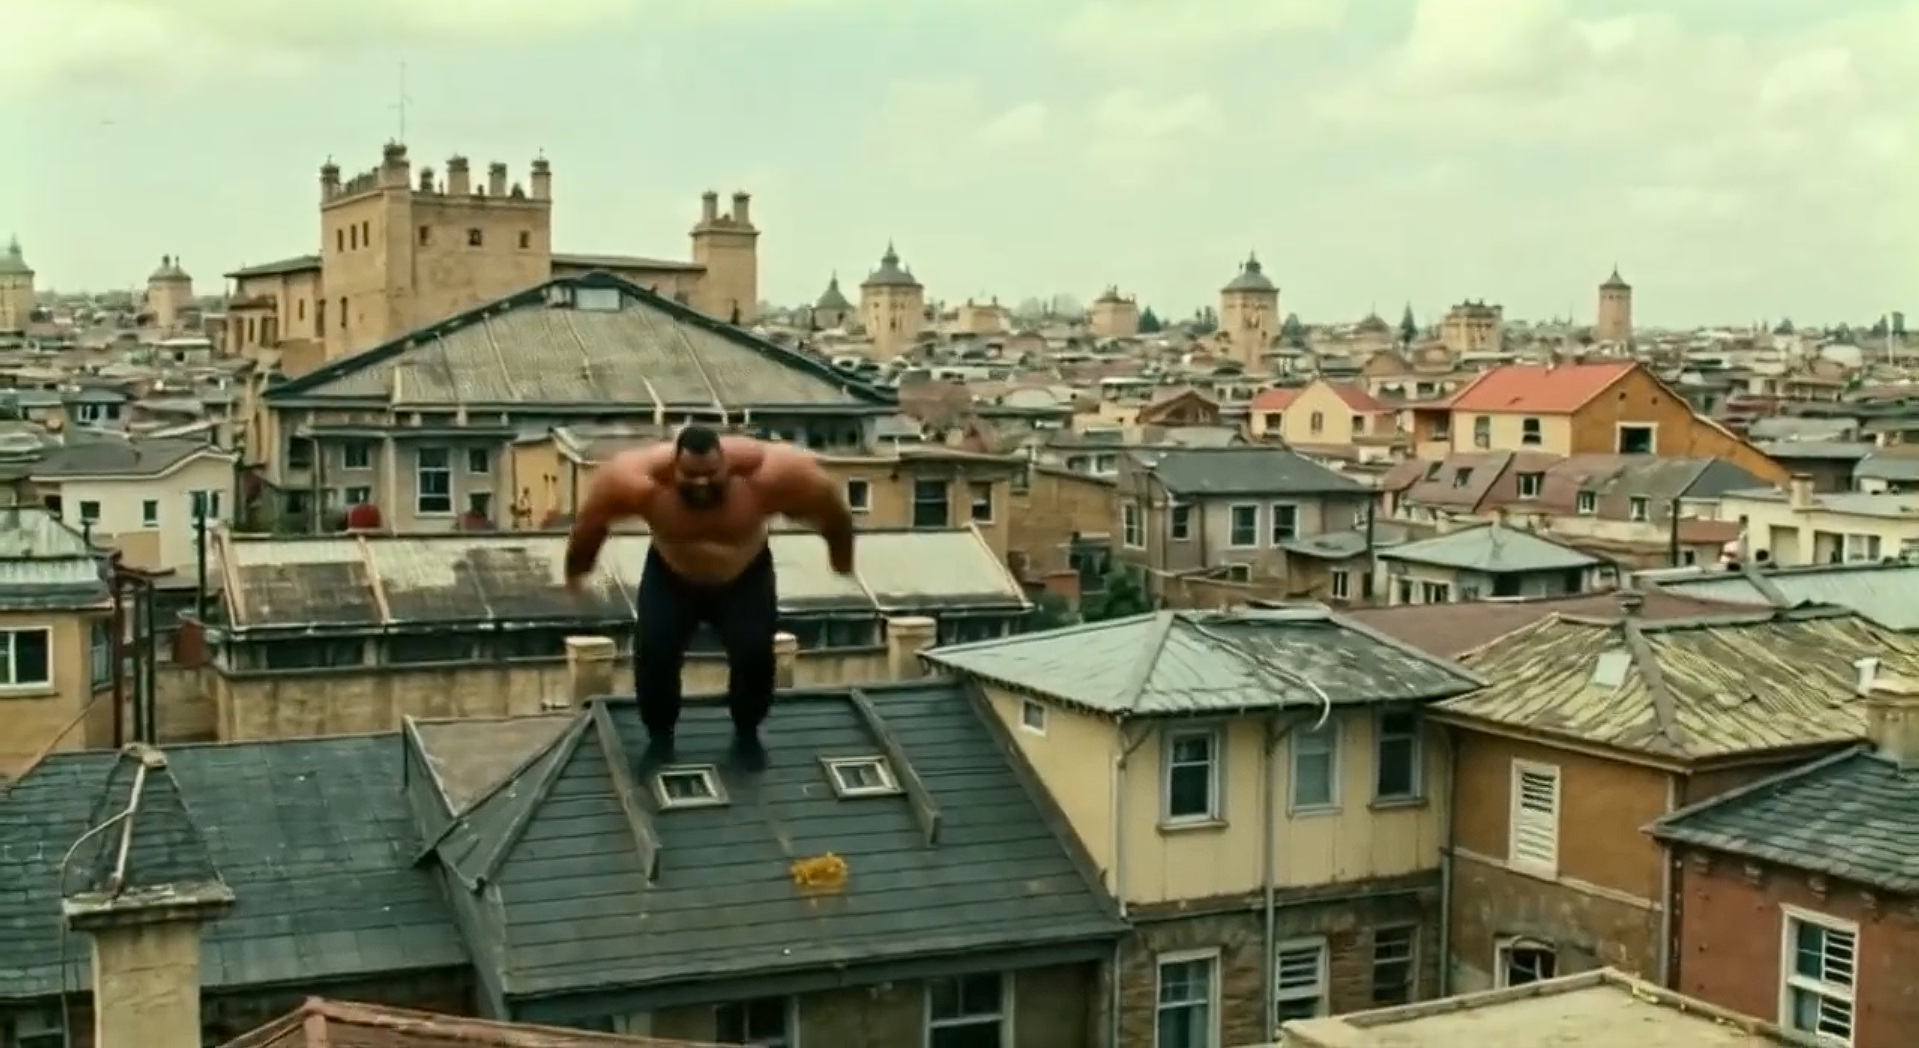
\includegraphics[width=\columnwidth]{image6.png}
    \caption{Incorrect sense of scale; impressive environment}
\end{figure}

For the second one:
\begin{figure}[t]
    \centering
    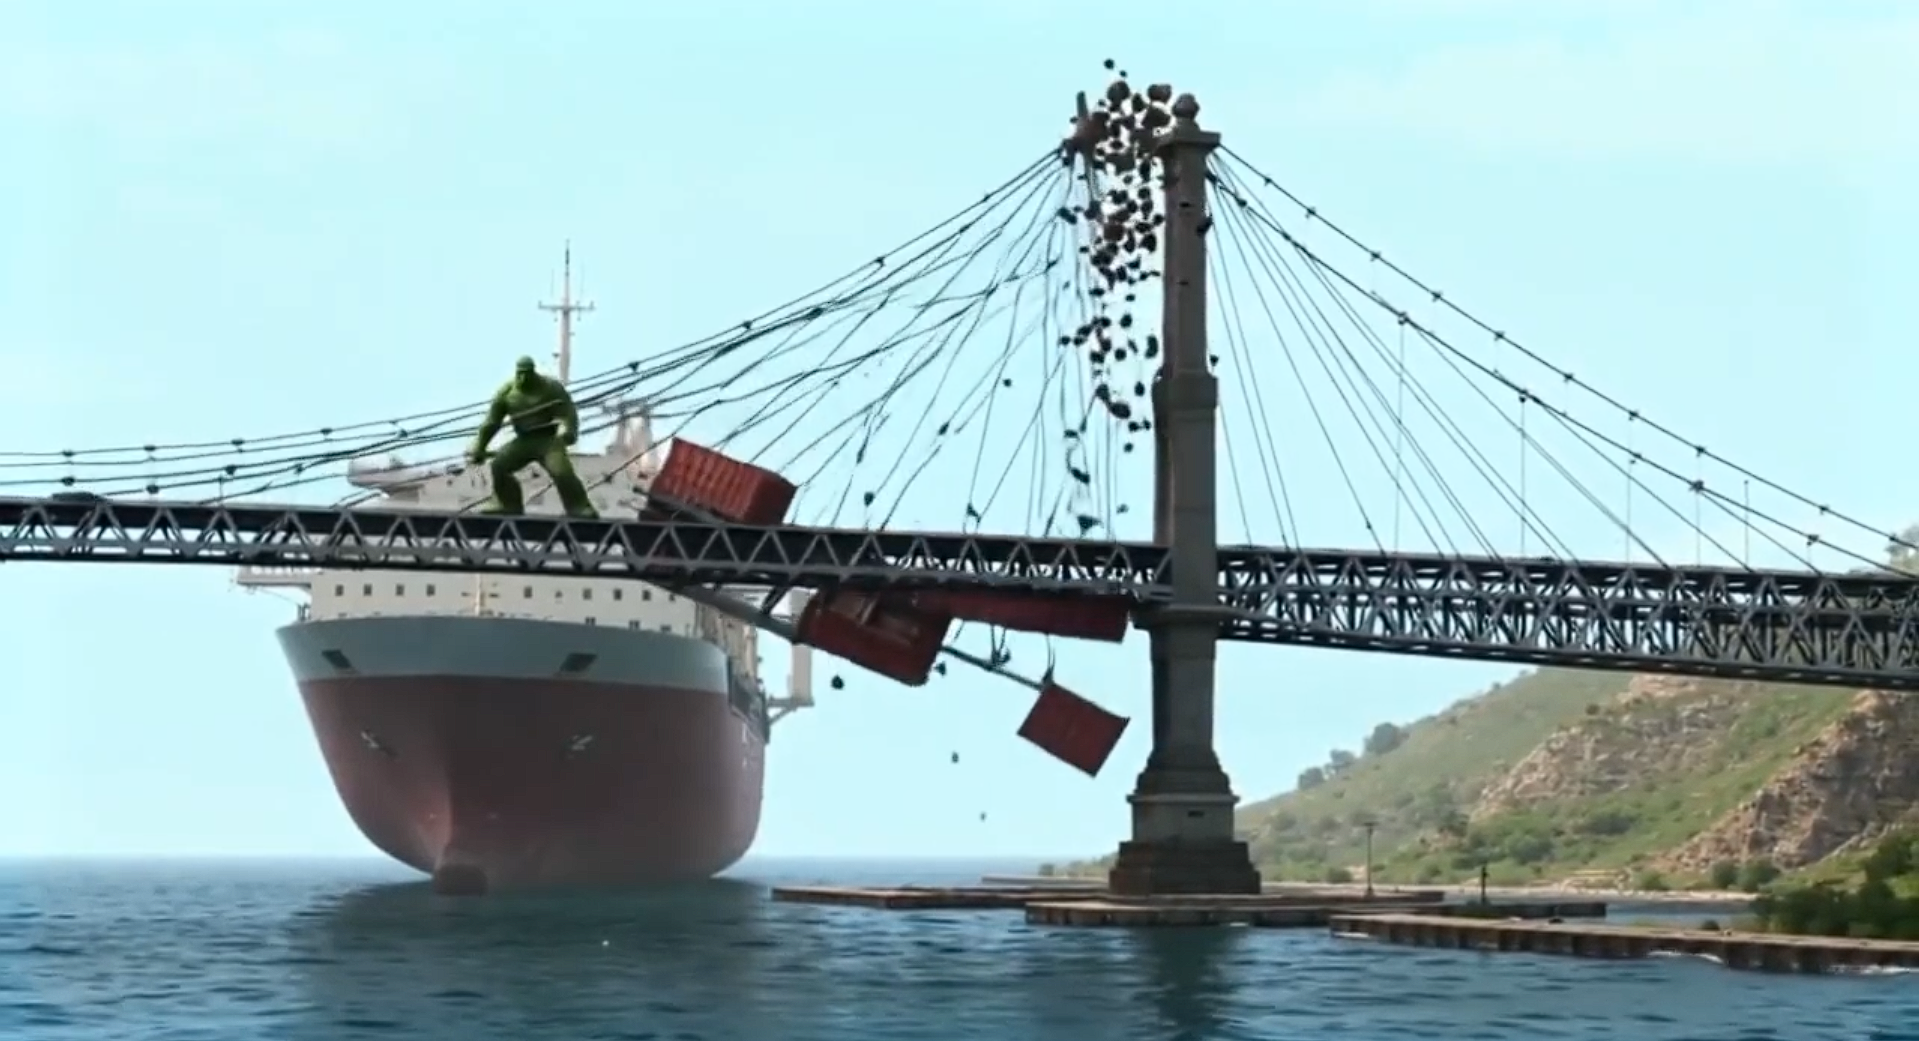
\includegraphics[width=\columnwidth]{image7.png}
    \caption{Extremely poor physical interactions, no reference to Godzilla}
\end{figure}

The third prompt:
\textbf{Missing}

The fourth prompt:
\begin{figure}[t]
    \centering
    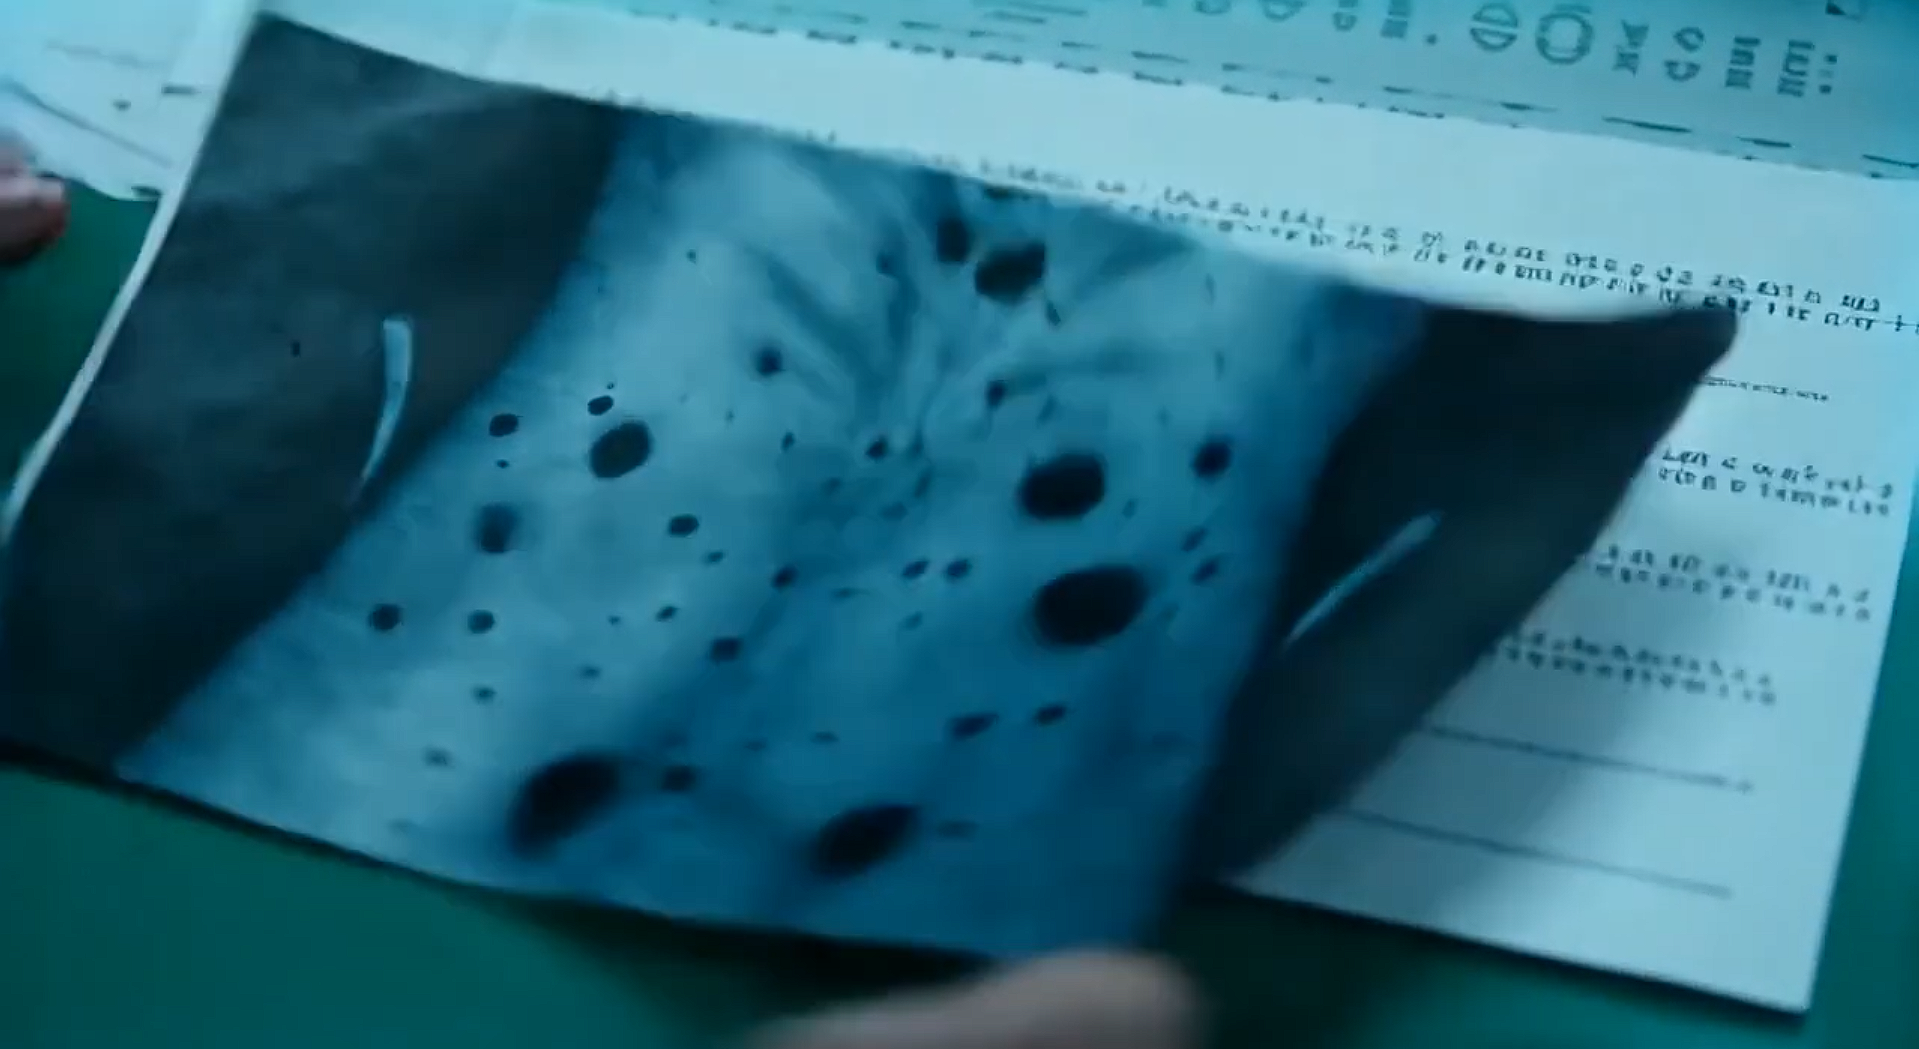
\includegraphics[width=\columnwidth]{image8.png}\\
    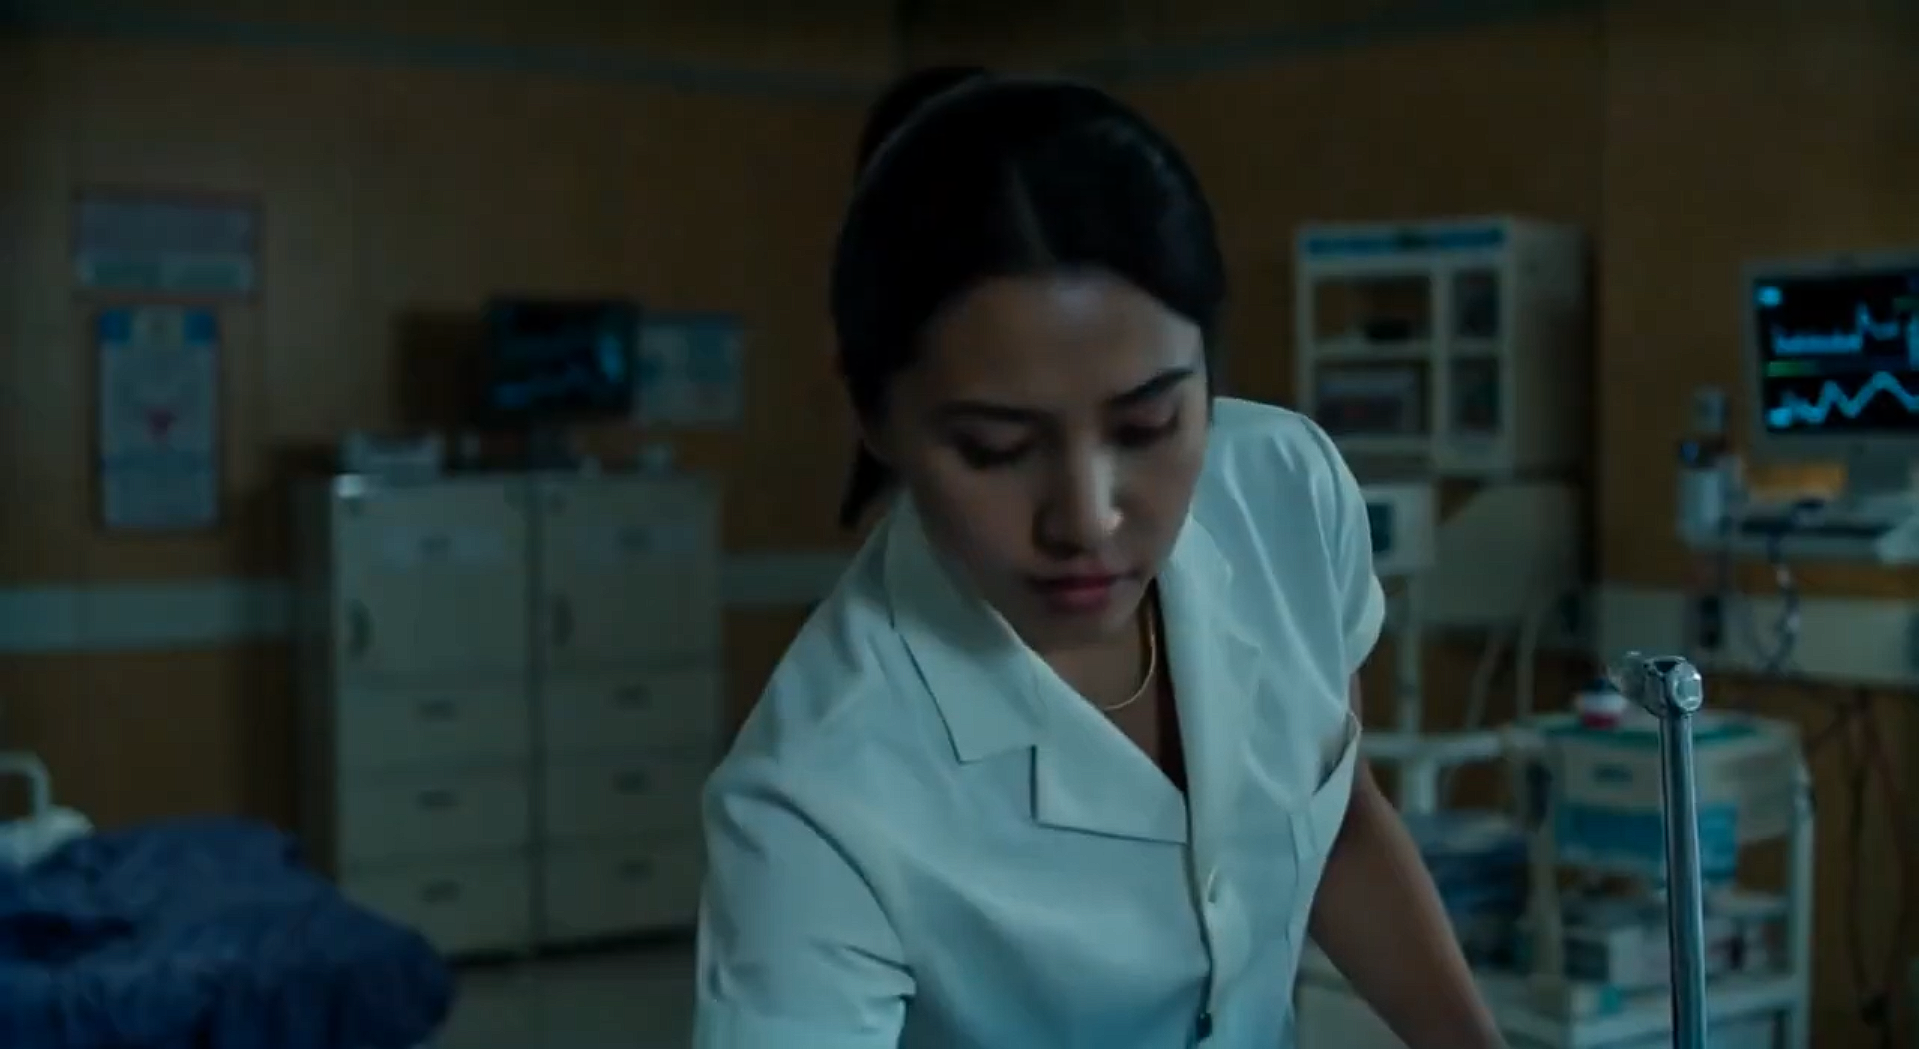
\includegraphics[width=\columnwidth]{image9.png}
    \caption{Gibberish text; high-quality animations; realistic person}
\end{figure}

The fifth prompt:
\begin{figure}[t]
    \centering
    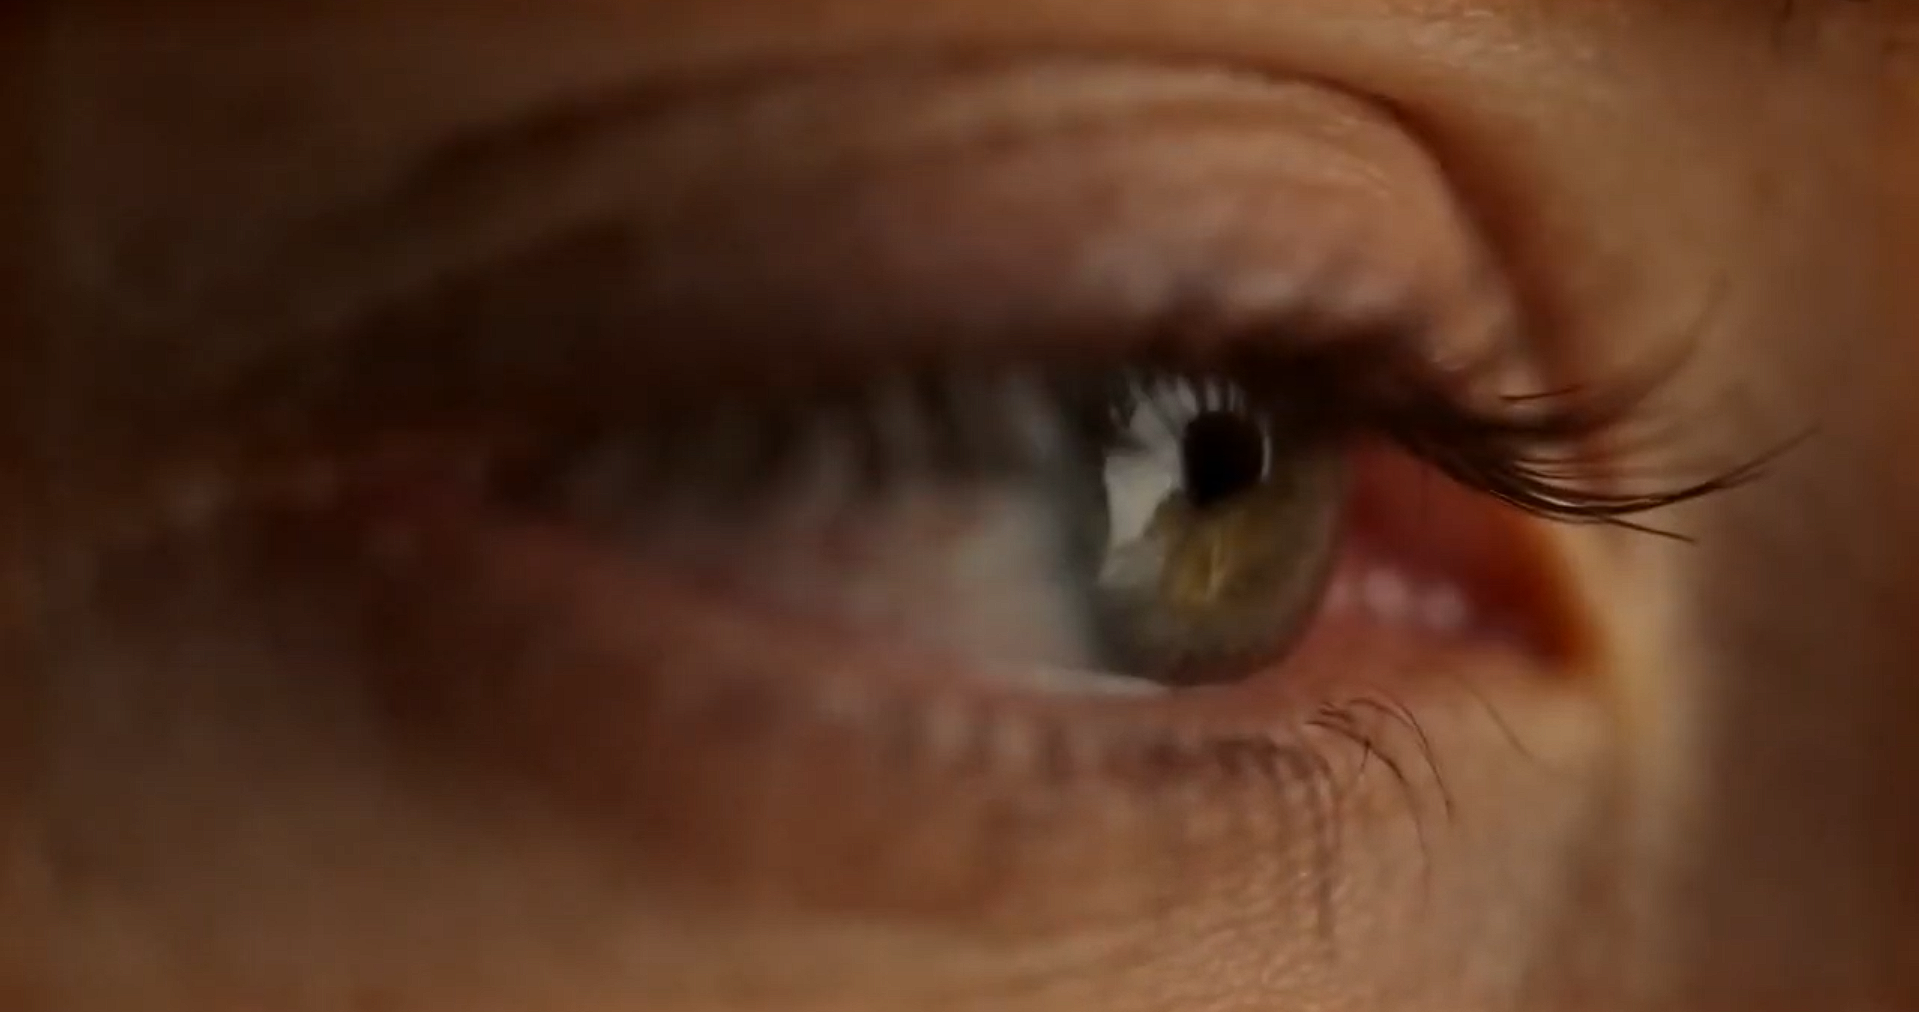
\includegraphics[width=\columnwidth]{image10.png}
    \caption{Photorealistic}
\end{figure}

The sixth prompt:
\begin{figure}[t]
    \centering
    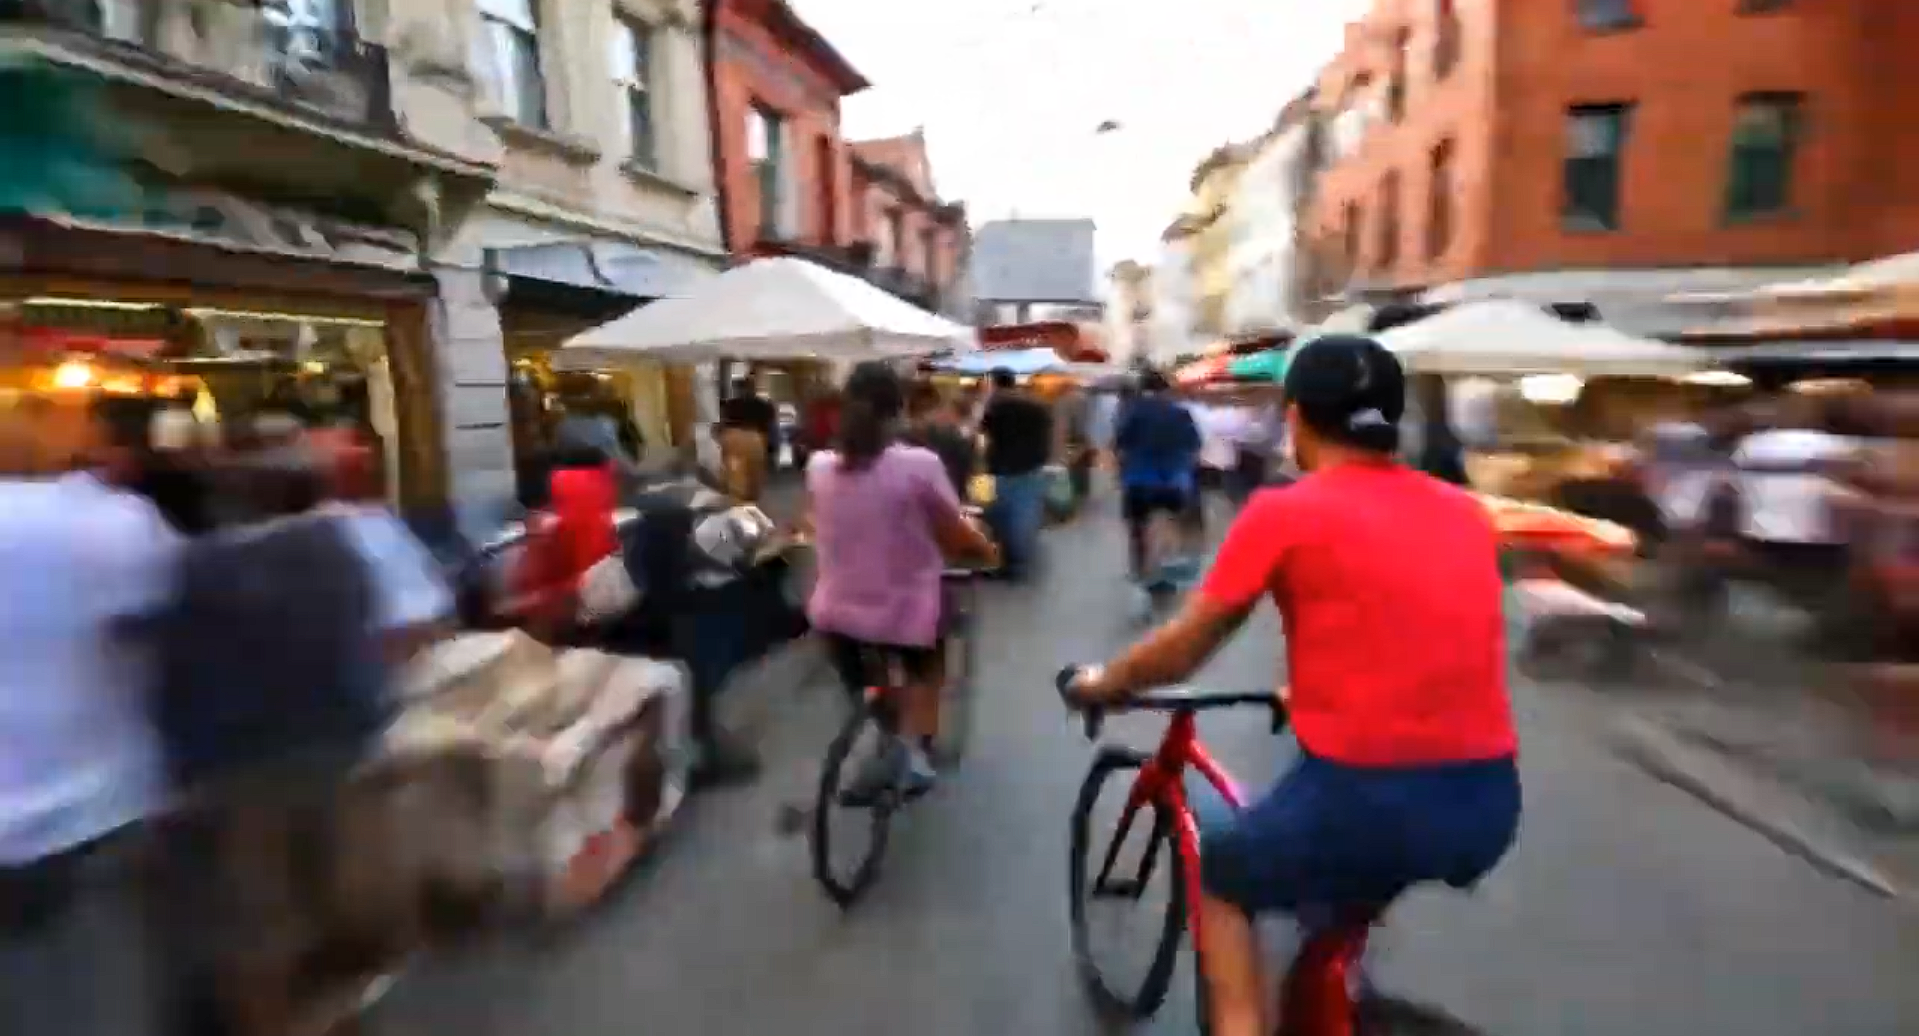
\includegraphics[width=\columnwidth]{image11.png}
    \caption{Believable environment work; cyclists move through people}
\end{figure}

\section{Wan 2.2 14B}
We now discuss the results of \verb|Wan 2.2|, the 14B parameter state-of-the-art model.

\subsection{Pinocchio}
One challenging aspect is to maintain the length of his nose and non human-like eyes. Wan 2.2 fails at maintaining the given eyes, but succeeds as inferring the former.

The first prompt:

\begin{figure}[t]
    \centering
    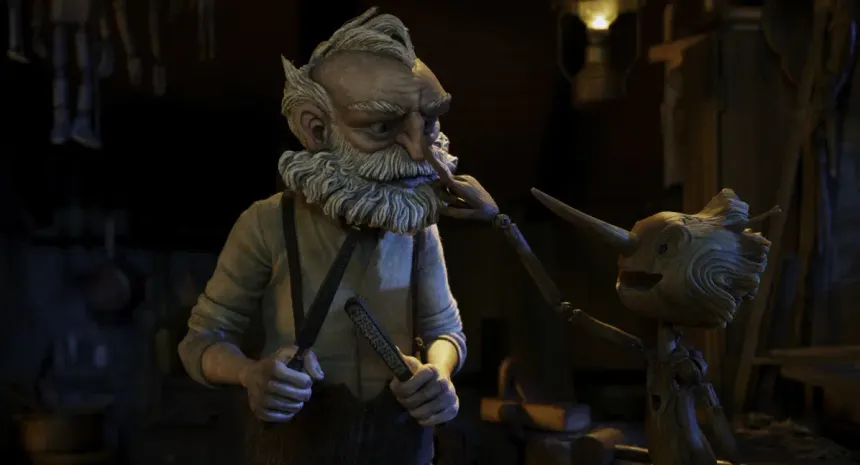
\includegraphics[width=0.48\columnwidth]{images/image5.png}\\
    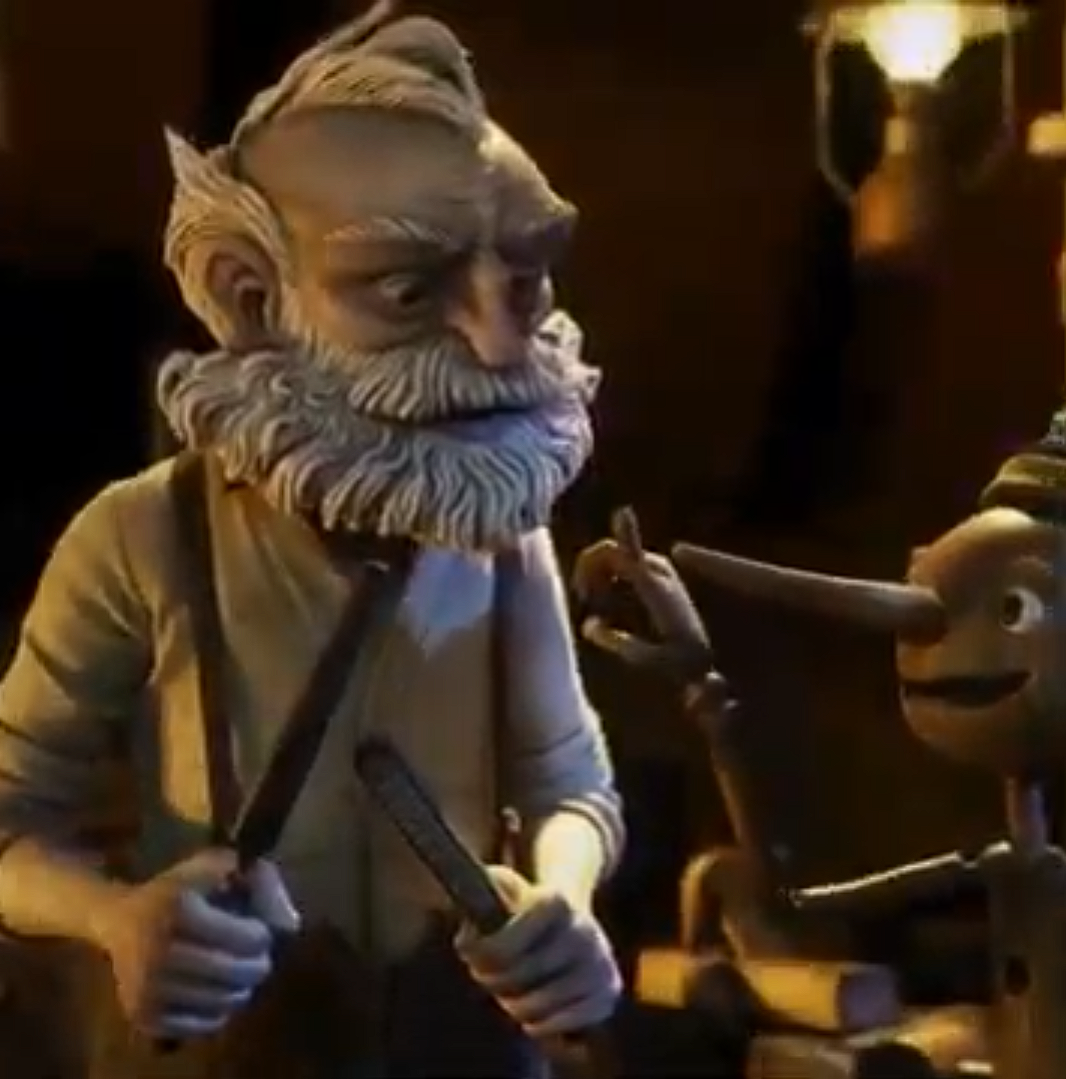
\includegraphics[width=0.48\columnwidth]{images/image4.png}\vspace{0.1\columnwidth}\\
    
\includegraphics[width=0.48\columnwidth]{images/image6.png}
    \caption{Incorrect eyes}
\end{figure}

\begin{figure}[t]
    \centering
    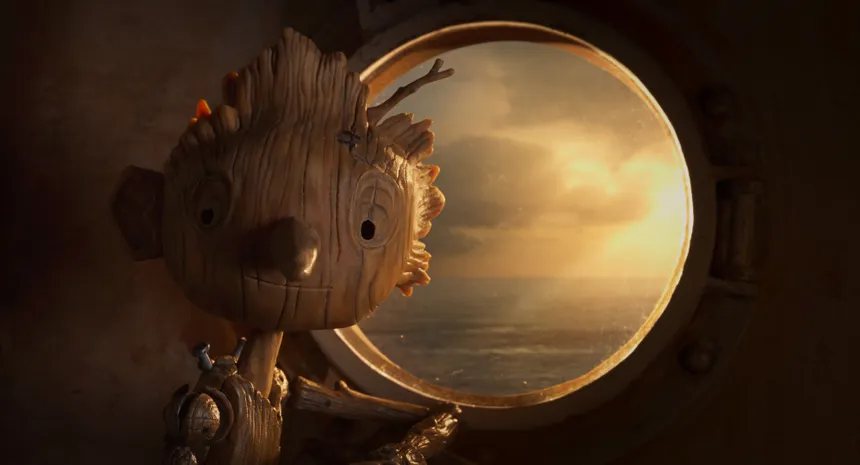
\includegraphics[width=0.48\columnwidth]{images/image2.png}\\
    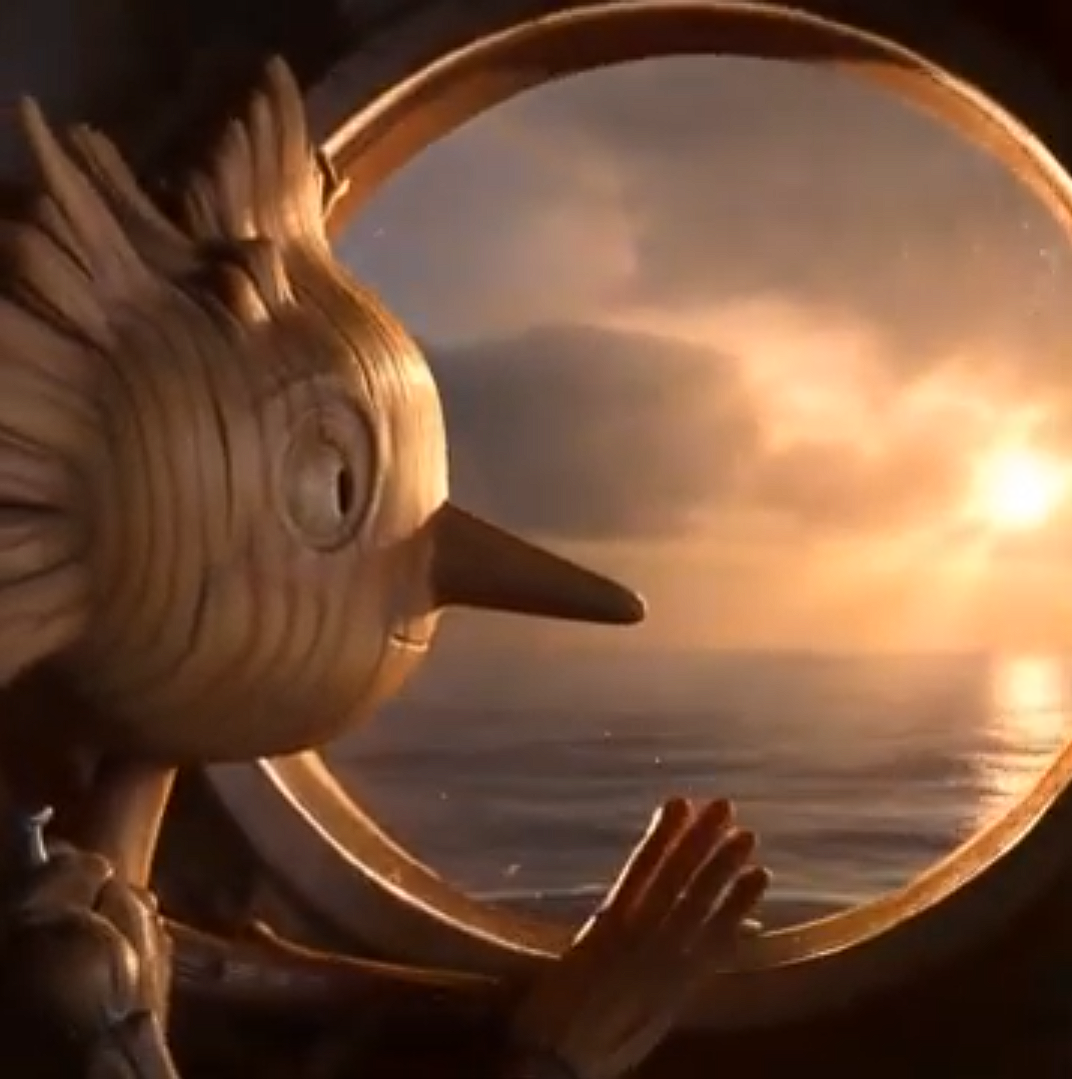
\includegraphics[width=0.48\columnwidth]{images/image1.png}\vspace{0.1\columnwidth}\\
    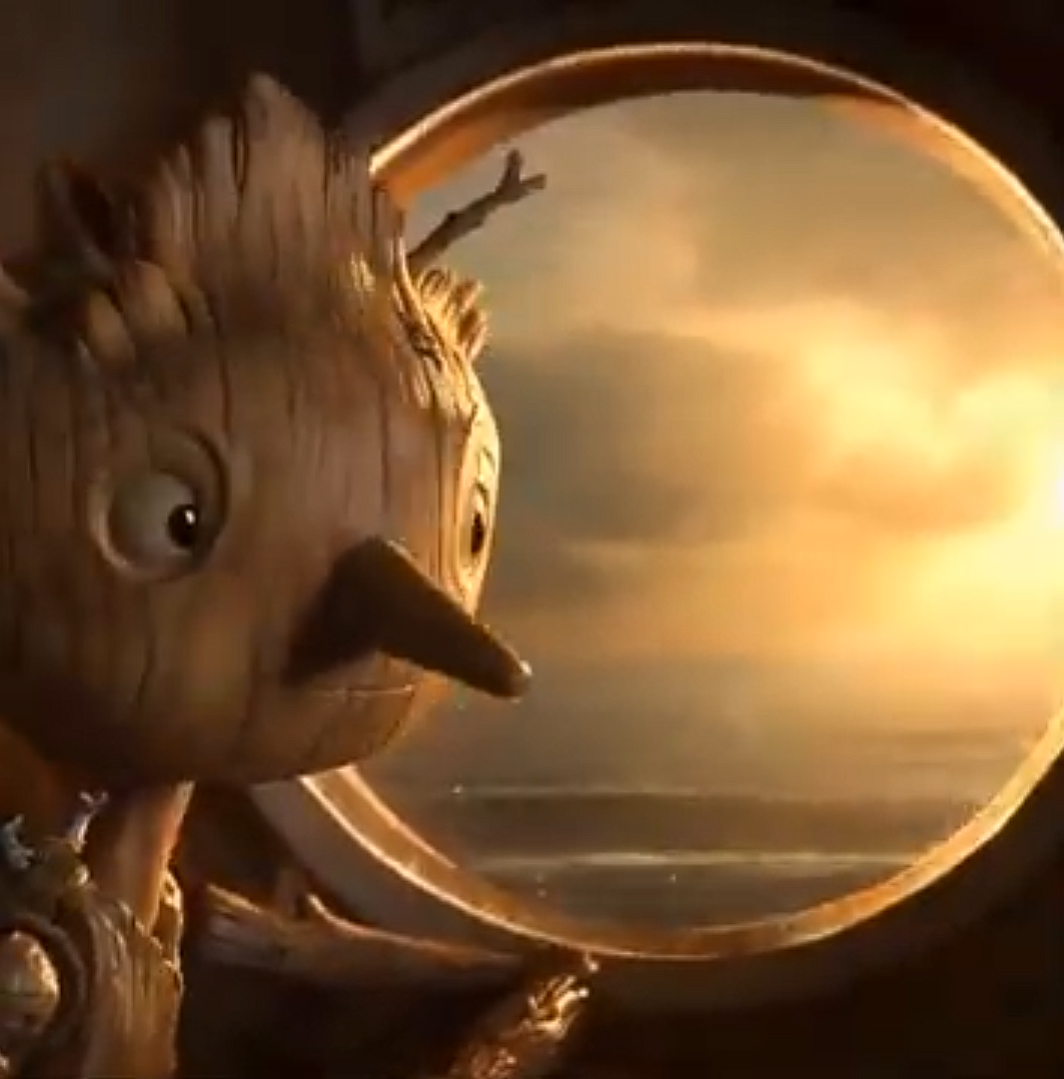
\includegraphics[width=0.48\columnwidth]{images/image3.png}
    \caption{Accurate nose (top: real)}
\end{figure}

\begin{acks}
    To Prof. Anoop, for premium access to ComfyUI.
\end{acks}

\bibliographystyle{ACM-Reference-Format}
\bibliography{sample-base}

\appendix

\section{Detailed prompts}
\subsection{Part 1: For image to video generation}
\subsection{Part 2: For text-to-image generation}

\section{Online Resources}

\end{document}